\title{LEZIONE 11 12/05/2020}\newline
\textbf{link} \href{https://web.microsoftstream.com/video/5bd1efee-fafa-4133-8e33-37fcd8b66da5}{clicca qui}
\subsection{Attrito dinamico o radente}
Nel momento in cui viene applicata una forza $F$ su un corpo e che la forza di attrito $T$ non è più in grado di bilanciarla si instaura un moto relativo fra i due corpi a contatto.\newline
\newline
Per verificare se si instaura o meno un moto relativo di usa la \textbf{verifica di aderenza}, cioè:
\[
    T \leq T_{lim} = f_s N
\]
Se questa disequazione si verifica siamo in presenza di \textbf{attrito statico}, se non si verifica siamo in condizione di \textbf{attrito dinamico}.\newline
\newline
In condizioni di attrito dinamico, il modello di Coulomb ci permette di stabilire la forza $T$ (o meglio $T_1$ e $T_2$ per effetto di azione-reazione) che viene scambiata fra i due corpi a contatto:\newline
[immagine dagli appunti del prof]
\begin{center}
    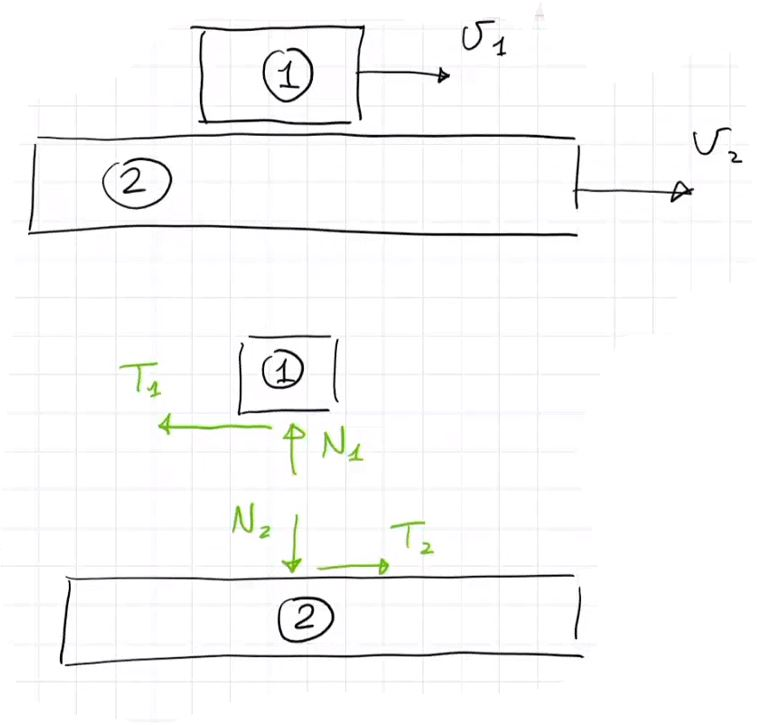
\includegraphics[height=3cm]{../lezione11/img1.JPG}
\end{center}
\[
    \begin{cases}
        \vec{T}_1 = - \vec{T}_2\\
        \vec{N}_1 = - \vec{N}_2
    \end{cases} \rightarrow \begin{cases}
        |\vec{T}_1| = |\vec{T}_2| = T\\
        |\vec{N}_1| = |\vec{N}_2| = N
    \end{cases}
\]
Possiamo ora definire la forza di attrito per il primo corpo come:
\[
    \vec{T}_1 = - f_d N  \frac{\vec{v}_{12}}{|\vec{v}_{12}|} = - f_d N  \frac{\vec{v}_1 - \vec{v}_2}{|\vec{v}_1 - \vec{v}_2|} 
\]
con $f_d$ \textbf{coefficiente di attrito dinamico}, e modulo $ |\vec{T}_1| = f_d N$, mentre direzione $ - \frac{\vec{v}_{12}}{|\vec{v}_{12}|}$ opposta alla velocità di strisciamente del corpo $1$ rispetto al copro $2$, che può essere espresso anche come $\frac{\vec{v}_1 - \vec{v}_2}{|\vec{v}_1 - \vec{v}_2|}$.\newline
[immaigne dagli appunti del prof]
\begin{center}
    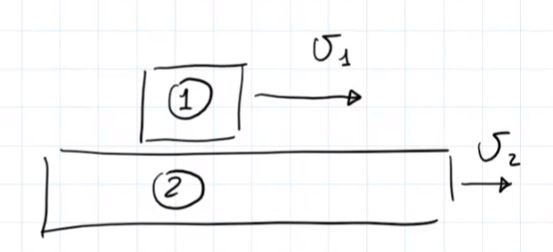
\includegraphics[height=3cm]{../lezione11/img2.JPG}
\end{center}
Notiamo inoltre che $\vec{v}_{12} = - \vec{v}_{21}$ e quindi la formula può essere riscritta come $\vec{T}_1 = f_d N  \frac{\vec{v}_{21}}{|\vec{v}_{21}|}$ .\newline
Porre molta attenzione a questo concetto di velocità relativa, la forza di attrito non dipende dalla velocità di uno solo dei due corpi, ma dalla velocità relativa di entrambi.
\ \newline
Operativamente il termine $N$ viene ricavato imponendo delle equazioni di equilibrio. Il termine $f_d$, che consideremo costante, dipende unicamente dai materiali a contatto, dalla finitura e dall'eventuale presenza di lubrificante. In realtà per velocità relative molto basse, il coefficiente di attrito dinamico non è costante e solitamente $f_d \leq f_s$.\newline
\newline
\subsubsection{Casi particolari}
Ipotiziamo che la velocità del corpo $2$ sia nulla: $\vec{v}_2 = 0$.\newline
[immaigne dagli appunti del prof]
\begin{center}
    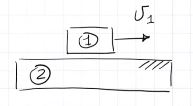
\includegraphics[height=3cm]{../lezione11/img3.JPG}
\end{center}
La forza di attrito sul corpo $1$ vale $|\vec{T}_1| = f_d N$ e la direzione sarà opposta alla velocità, cioè direzione $- \frac{\vec{v}_1}{|\vec{v}_1|}$. Sul secondo corpo quindi apparirà una forza uguale e contraria.\newline
[immagine dagli appunti del prof]
\begin{center}
    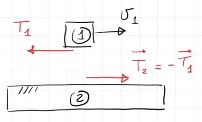
\includegraphics[height=3cm]{../lezione11/img4.JPG}
\end{center}
\ \newline
Ipotiziamo ora il caso contrario, cioè quello in cui $\vec{v}_1 = 0$:\newline
[immagine dagli appunti del prof]
\begin{center}
    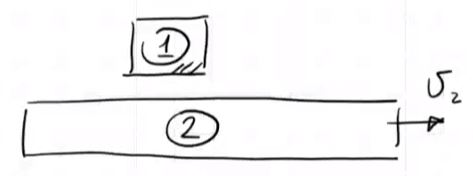
\includegraphics[height=3cm]{../lezione11/img5.JPG}
\end{center}
In questo caso, abbiamo sempre $|\vec{T}_1| = f_d N$, ma la direzione sarà contraria alla direzione di $\vec{v}_{12} = \vec{v}_1 - \vec{v}_2 = - \vec{v}_2$, per cui $\vec{T}_1 = - f_d N \frac{\vec{v}_2}{|\vec{v}_2|}$, quindi in questo caso $T_1$ avrà direzione concorde con $v_2$:\newline
[immagine dagli appunti del prof]
\begin{center}
    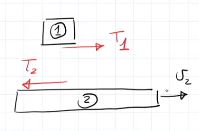
\includegraphics[height=3cm]{../lezione11/img6.JPG}
\end{center}
\ \newline
Vediamo ora un caso più generale, in cui $v_1 > v_2$:\newline
[immagine dagli appunti del prof]
\begin{center}
    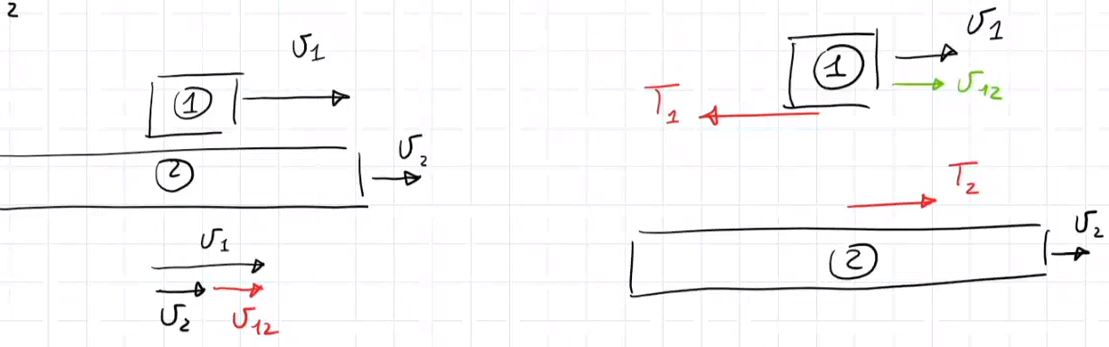
\includegraphics[height=3cm]{../lezione11/img7.JPG}
\end{center}
\ \newline
Nel caso in cui si abbia $\vec{v}_1 = \vec{v}_2$, allora non si ha moto relativo fra i due corpi, quindi si ha attrito statico.
\subsection{Potenza legata alle forze d'attrito}
La potenza legata alle forze d'attrito è sempre una \textbf{potenza dissipata}.\newline
\newline
Vediamo come calcolarla:
\[
    W_d = \vec{T}_1 \;\text{x}\;\vec{v}_1 + \vec{T}_2 \;\text{x}\; \vec{v}_2 + \cancel{\vec{N}_1 \;\text{x}\;\vec{v}_1} + \cancel{\vec{N}_2 \;\text{x}\; \vec{v}_2} 
\]
In cui i termini cancellati sono prodotti vettoriali fra vettori perpendicolari.\newline
Inoltre sapendoche $\vec{T}_2 = - \vec{T}_1$ possiamo scrivere:
\[
    W_d = \vec{T}_1 \; \text{x}\; (\vec{v}_1 - \vec{v}_2) = \vec{T}_1 \;\text{x}\; \vec{v}_{12} = - f_d N \frac{\vec{v}_{12}}{|\vec{v}_{12}|} \;\text{x}\;\vec{v}_{12}
\]
\[
    W_d = - f_d N \frac{v_{12}^2}{|\vec{v}_{12}|} = f_d N |v_{12}|
\]
Siccome $f_d N > 0$ e $|v_{12}| > 0$, allora $- f_d N |v_{12}| <0$, da cui ricaviamo che si tratta di potenza dissipata.
\subsection{Attrito per un disco che rotola su una guida piana}
[immagine dagli appunti del prof]
\begin{center}
    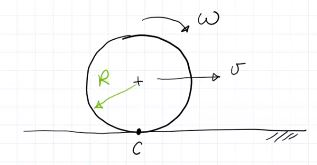
\includegraphics[height=3cm]{../lezione11/img8.JPG}
\end{center}
Considerando i corpi rigidi, il contatto fra disco e piano è di tipo puntiforme e avviene nel punto $C$. Isoliamo i due corpi e notiamo e mostriamo le forze di azione e reazione:\newline
[immagine dagli appunti del prof]
\begin{center}
    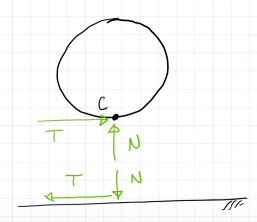
\includegraphics[height=3cm]{../lezione11/img9.JPG}
\end{center}
A questo punto dobbiamo distinguere due casi separati:
\begin{itemize}
    \item \textbf{Puro rotolamento}: Nel caso di puro rotolamento il punto $C$ rappresenta il centro di istantaneo rotolamento, per cui $\vec{v}_C = 0$ e quindi non vi è moto relativo, dunque siamo in condizioni di attrito statico. In questo caso il sistema ha $1$ grado di libertà, il rotolamento.
    \item \textbf{Strisciamento}: In questo caso siamo in presenza di un moto relativo fra i due corpi, e di conseguenza di attrito dinamico. In questo sistema si hanno $2$ gradi di libertà, rotolamento e strisciamento.
\end{itemize}
\ \newline
In pratica, quando stiamo studiando un disco che rotola, dobbiamo ipotizzare le condizioni di puro rotolamento, calcolare le forze $T$ e $N$, imponendo delle equazioni di equilibrio dinamico e infine si verifica la condizione di aderenza, cioè $T \leq T_{lim} = f_s N$. Se questa disuguaglianza è verificata, allora l'ipotesi fatta è corretta, altrimenti le ipotesi sono scorrette, quindi abbiamo moto relativo fra i due corpi (strisciamneto) e saremo in condizioni di attrito dinamico, e quindi i valori di $T$ e $N$ calcolati non vanno bene ($|\vec{T}| = f_d |\vec{N}|$).\newline
\newline
Se siamo in condizione di strisciamento, avremo della potenza dissipata.\newline
Se siamo in condizioni di puro rotolamento, le forze $T$ e $N$ sono applicate al punto $C$, che ha velocità nulla, quindi la potenza dissipata per attrito si annulla:
\[
    W_d = (\vec{T} + \vec{N}) \;\text{x}\; \vec{v}_C = 0
\]
Sperimentalmente però questo risultato non torna, il problema sta nel modello di Coulomb che stiamo utilizzando. Per far fronte a questo problema si utilizza il modello di resistenza al rotolamento.
\subsubsection*{Modello di resistenza al rotolamento}
L'ipotesi alla base di questo modello è che si deve essere in condizioni di puro rotolamento e quindi di attrito statico. Il modello prevede di usare come punto di applicazione della forza $N$, non il punto $C$ di istantanea rotazione, ma un punto $C'$ in avanti di una quantità $u$ rispetto alla direzione del moto del disco.\newline
[immagine dagli appunti del prof]
\begin{center}
    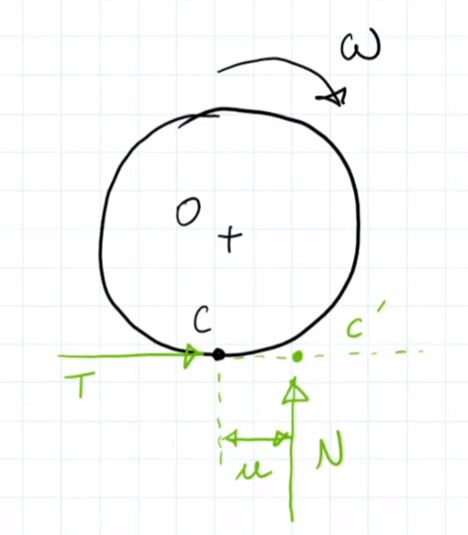
\includegraphics[height=3cm]{../lezione11/img10.JPG}
\end{center}
Interpretando così il punto di applicazione della forza $N$, posso ora spostare nuovamente nel punto $C$ questa forza, aggiungendo ora una componente di momento detto \textbf{momento di trasporto} $C_r$, pari a $N$ moltiplicata per il braccio $u$, questa coppia si oppone alla rotazione del disco e quindi dissipa energia:
\[
    W_d = \vec{C}_r \;\text{x}\; \vec{\omega} = -C_r \omega = - N u \omega < 0
\]
[immagine dagli appunti del prof]
\begin{center}
    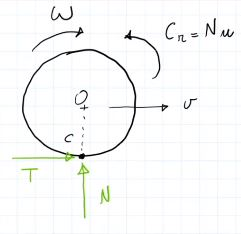
\includegraphics[height=3cm]{../lezione11/img11.JPG }
\end{center}
Generalmente la quantità $u$, cioè la distanza fra $C$ e $C'$, viene espressa in dipendenza del \textbf{coefficiente di attrito evolvente} e del raggio $R$ del disco:
\[
    u = f_v R
\]
Possiamo quindi riscrivere la potenza dissipata come
\[
    W_d = - N u \omega = - N f_v R \omega = - N f_v R \frac{v}{R} = - N f_v v
\]
dove abbiamo considerato che $v = \omega R$ nel moto rotatorio.
\subsection{Bilancio di Potenze (BdP) con attriti}
Quando abbiamo parlato di bilancio di potenze abbiamo fatto come ipotesi che i vincoli fossero perfetti, cioè lisci e senza attrito.\newline
\newline
Per estendere il bilancio di potenze e il teorema dell'energia cinetica a vincoli non perfetti ci basta aggiungere al bilancio di potenza la potenza dissipata dalle forze d'attrito:
\[
    W = W_d + W_{in} = 0
\]
dove sicuramente $W_d$ sarà negativa.\newline
Il teorema dell'energia cinetica sarà invece:
\[
    W + W_d = \frac{dE_c}{dt}
\]
Queste equazioni sono quindi valide per \textbf{vincoli fissi e bilateri} (non perfetti).
